\documentclass[a4paper]{llncs}

\usepackage{amssymb}
\setcounter{tocdepth}{3}
\usepackage{graphicx}

\usepackage{url}
\urldef{\mailsa}\path|{v.bajpai, j.schoenwaelder}@jacobs-university.de|
\newcommand{\keywords}[1]{\par\addvspace\baselineskip
\noindent\keywordname\enspace\ignorespaces#1}

% added by Vaibhav
%----------------------------------------------------------------------
\usepackage[utf8]{inputenc}
\usepackage[T1]{fontenc}
\usepackage[nolist]{acronym}
\renewcommand{\ttdefault}{cmtt}
\usepackage{cite}
%----------------------------------------------------------------------


\begin{acronym}
  \acro{RIR}{Regional Internet Registry}
  \acro{NETCONF}{Network Configuration}
  \acro{CGN}{Carrier-Grade NAT}
  \acro{NAT}{Network Address Translation}
  \acro{FCC}{Federal Communications Commission}
  \acro{RIPE NCC}{RIPE Network Coordination Centre}
  \acro{RTT}{round-trip time}
  \acro{M-Lab}{Measurement Lab}
  \acro{CDN}{Content Delivery Network}
  \acro{ISP}{Internet Service Provider}
  \acro{MA}{Measurement Agent}
  \acro{QoE}{Quality of Experience}
\end{acronym}

\begin{document}

\mainmatter  % start of an individual contribution

% first the title is needed
\title{Understanding the Impact of Network Infrastructure Changes using
Large-Scale Measurement Platforms}


\author{Vaibhav Bajpai \and Jürgen Schönwälder%
\thanks{This work was supported by the European Community’s Seventh Framework
Programme (FP7/2007-2013) grant no. 317647 (Leone)}}
\institute{Computer Science, Jacobs University Bremen, Germany\\
\mailsa}
\maketitle

\begin{abstract}

A number of large-scale measurement platforms have emerged in the last few
years. These platforms have deployed thousands of probes within the access,
backbone networks and at residential gateways.  Their primary goal is to
measure the performance of broadband access networks and to help regulators
sketch better policy decisions. We want to expand the goal further by using
large-scale measurement platforms to understand the impact of network
infrastructure changes.

\end{abstract}


% sections
%----------------------------------------------------------------------
\section{Research Statement}
An interest to understand the evolution of the Internet from the user' vantage
point started with establishing techniques to remotely probe the broadband
links. Dischinger \emph{et al.} in \cite{dischinger:2007} for instance, inject
packet trains and use the responses received from gateway to infer the
broadband link characteristics. This led to development of a number of
software-based solutions, \texttt{netalyzr} \cite{kreibich:2010}, for
instance, that require explicit interactions with the broadband consumer.
Recently, the requirement for accurate measurements, coupled with \ac{FCC}'
initiated efforts to define data-driven standards has led to the deployment of
a number of large-scale measurement platforms that perform measurements using
dedicated hardware probes not only from within the ISP' network but also
directly from the home gateway. 

In a recent study, sponsered by the \ac{FCC}, Sundaresan \emph{et al.}
\cite{sundaresan:2011} have used such a measurement data from a swarm of
deployed SamKnows probes to investigate the throughput and latency of access
network links across multiple ISPs. in the United States. They have coupled
this data with their own Bismark platform \cite{sundaresan:2012} to also
investigate different traffic shaping policies enforced by the ISP and to
understand the bufferbloat phenomenon. The empirical findings of this study
has recently been repraised by Canadi \emph{et al.} in \cite{canadi:2012}
where they use crowdsourced data from \url{speedtest.net} to compare both
results. The primary aim is to measure the performance and reliability of
broadband access networks and facilitate the regulators with research findings
to help them make policy decisions that eliminate the ISP' monopoly
\cite{draft-schulzrinne-lmap-requirements-00}.  As a result, the focus is on
defining metrics and implement measurement tests that help achieve this goal.

In the past, we have performed an experimental evaluation of IPv6
transitioning technologies to identify how well current applications and
protocols interoperate with them \cite{vbajpai:2012}. Using a large-scale
measurement platform we want to take this further and study the IPv6 evolution
and its repercussions. We want to describe metrics and implement measurement
tests that help us answer questions of the form:

\begin{itemize}
  \item \emph{How does the performance of IPv6 compare to that of IPv4 in real world?}
  \item \emph{Can we identify deployment of \ac{CGN} from a gateway?}
  \item \emph{Can we identify deployments of multiple layers of NAT from a gateway?}
  \item \emph{How much do services centralize on core \ac{CDN}s?}
  \item \emph{To what extend does the network experience depend on
              localized data?}
\end{itemize}

%In our preliminary study, we have witnessed that a major portion of the
%services in practicality centralize either on core content delivery networks
%or major cloud platforms.
\label{sec:rstatement}
\section{Proposed Approach}
% samknows and bismark
SamKnows\footnote{\url{http://www.samknows.com}} specializes in the deployment
of hardware-based probes that perform measurements to assess the performance
of broadband access networks. The probes function by performing active
measurements when the user is not aggressively using the network.  RIPE
Atlas\footnote{\url{https://atlas.ripe.net}} is another independent
measurement infrastructure deployed by the \ac{RIPE NCC}. It consists of
thousands of hardware probes distributed around the globe that perform
\ac{RTT} and traceroute measurements to a number of preconfigured destinations
alongside DNS queries to DNS root servers.

% measurement lab
\ac{M-Lab} \cite{dovrolis:2010} is an open, distributed platform to deploy
Internet measurement tools. The measurement results are stored on Google's
infrastructure. The tools vary from measuring TCP throughput and available
bandwidth to emulating clients to identify end-user traffic differentiation
policies \cite{dischinger:2010, kanuparthy:2011} to performing reverse
traceroute lookups from arbitrary destinations \cite{bassett:2010}.

% leone
It will only be possible to answer the aforementioned research questions with
access to a large-scale measurement platform. As partners of the Leone
consortium, we will leverage the infrastructure of our partners. We will
define metrics particularly targeted to our research questions and complement
them by implementing subsequent measurement tests. The developed measurement
tests will be deployed in our partner's networks, but may also become part of
SamKnows global infrastructure. The SamKnows infrastructure already has
several thousand deployed probes and will continue to grow during the
project's lifetime. The collected data will be conglomerated from multiple
measurement points and finally analyzed to uncover information needed to help
us answer these questions. This requires to develop data analysis algorithms
that can integrate data from different data sources such as address block
allocations from \ac{RIR}s or prefix and path information from BGP route
views. In this pursuit, we have started with a study to assess how the user
experience is effected by the deployment of IPv6.
\label{sec:approach}
\section{Preliminary Results}
\begin{figure}[t]
  \begin{minipage}[t]{0.50\textwidth}
    \centering
    \resizebox*{1.0\textwidth}{!}{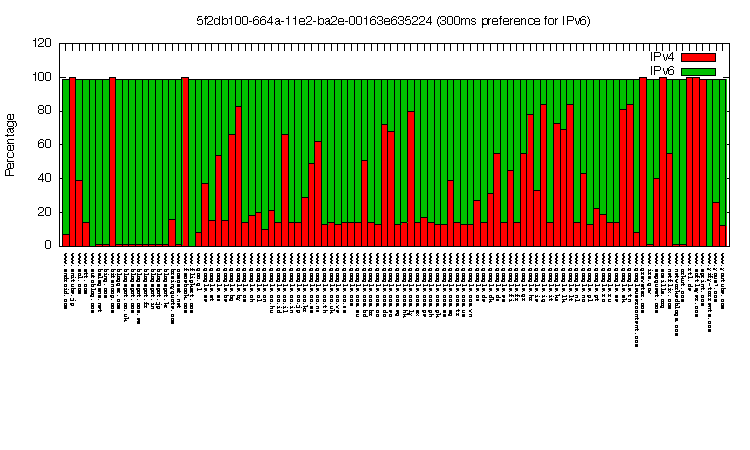
\includegraphics{figures/t28971-competition-300ms}}
    \caption{Native IPv4 and Teredo Tunnel}
  \end{minipage}
  \begin{minipage}[t]{0.50\textwidth}
    \centering
    \resizebox*{1.0\textwidth}{!}{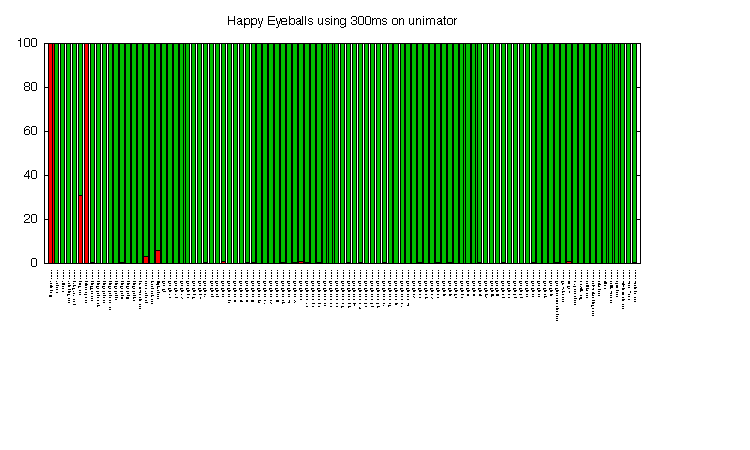
\includegraphics{figures/unimator2-competition-300ms}}
    \caption{Native IPv4 and Native IPv6}
  \end{minipage}
\caption{\label{fig:happy-v4-v6-compete}IPv4 and IPv6 Happy Eyeball Competition} 
\end{figure}

A user when attempting to connect to a dual-stacked web service prefers
connecting over IPv6. This is because in POSIX systems, the domain name
resolution system call \texttt{getaddrinfo(\ldots)} returns a list of
endpoints in an order that prioritizes an IPv6-upgrade path \cite{rfc6724}.
The dictated order can dramatically reduce the application responsiveness in
situations where IPv6 connectivity is broken. This is because, the attempt to
connect over an IPv4 endpoint will take place only when the IPv6 connection
attempt has timed out, which can be in the order of seconds.

\begin{figure}[t]
  \begin{minipage}[t]{0.50\textwidth}
    \centering
    \resizebox*{1.0\textwidth}{!}{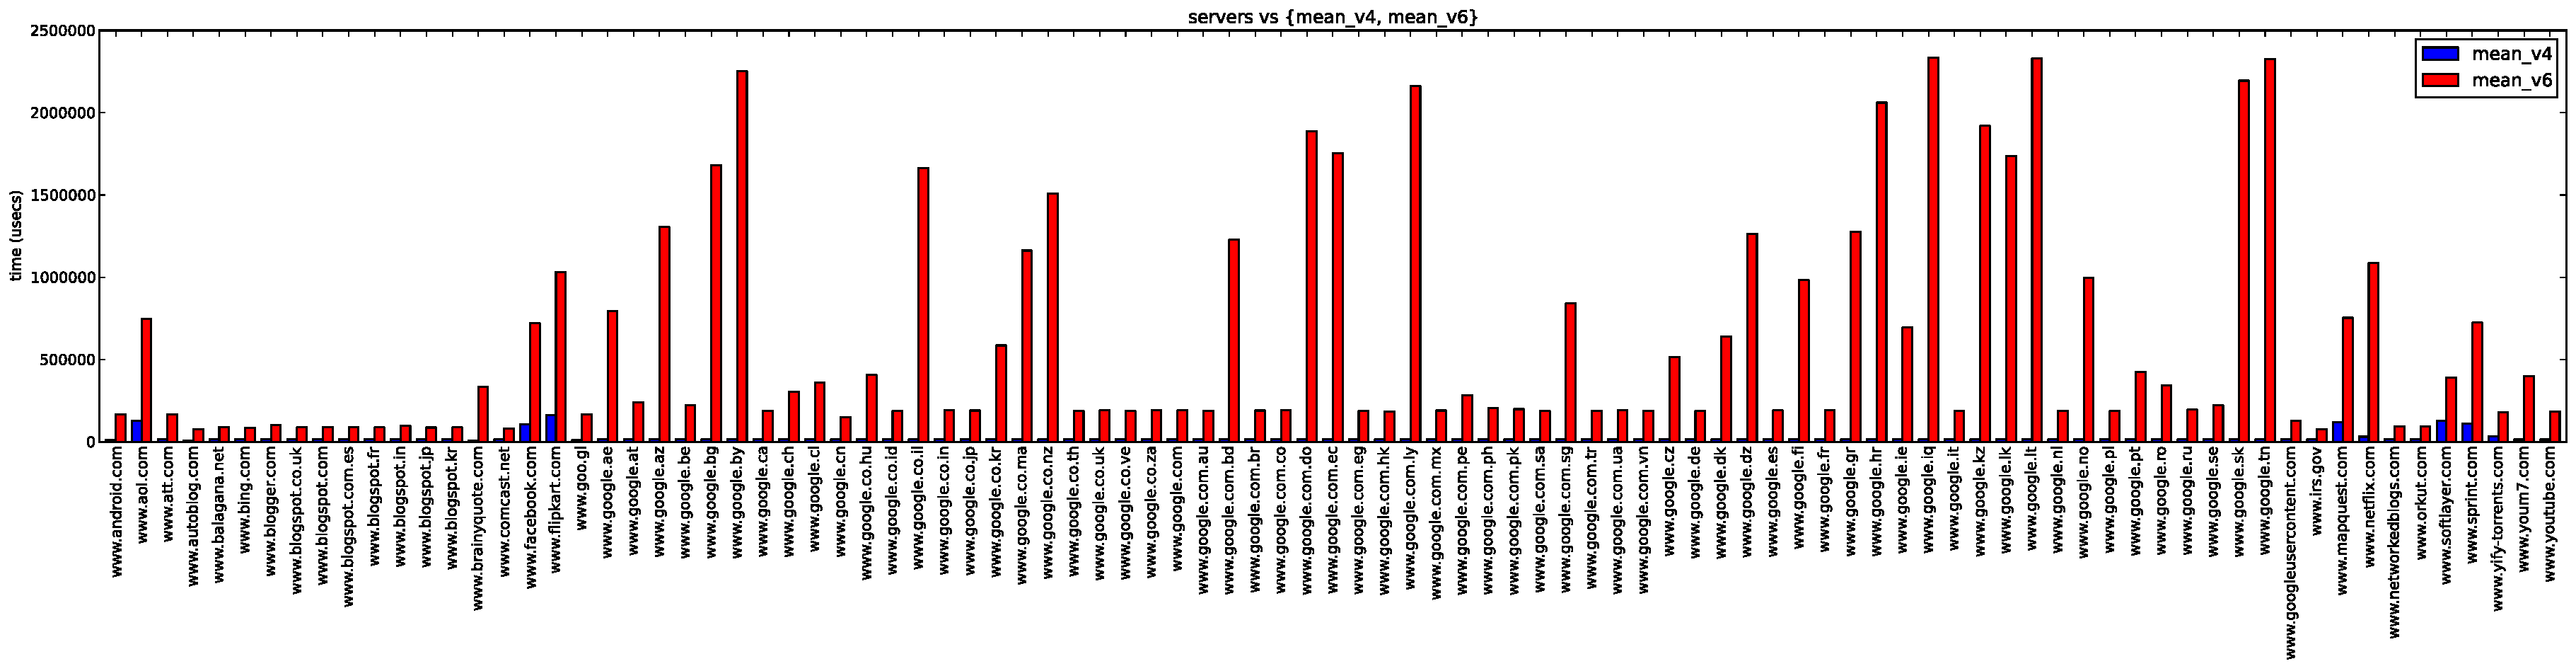
\includegraphics{figures/t28971-mean}}
    \caption{Native IPv4 and Teredo Tunnel}
  \end{minipage}
  \begin{minipage}[t]{0.50\textwidth}
    \centering
    \resizebox*{1.0\textwidth}{!}{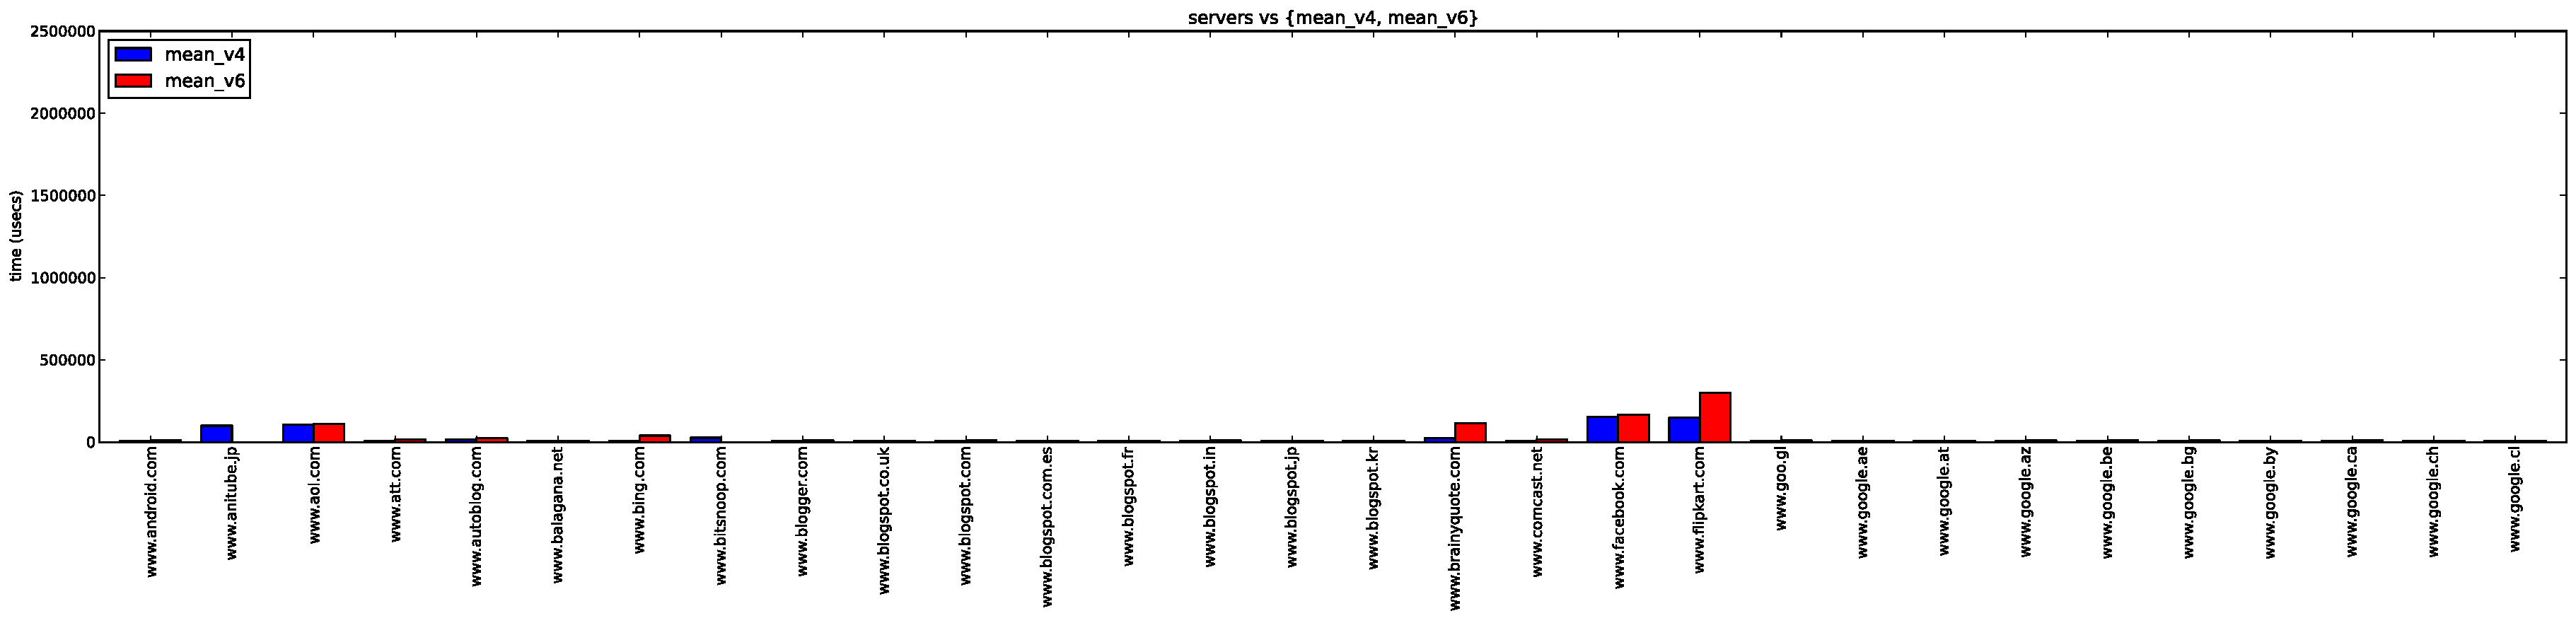
\includegraphics{figures/unimator2-mean}}
    \caption{Native IPv4 and Native IPv6}
  \end{minipage}
\caption{\label{fig:happy-v4-v6-mean-std} Mean and Standard Deviations for
IPv4 and IPv6}
\end{figure}

This noticeable degraded user experience can be subverted by making
applications apply the happy eyeballs algorithm \cite{rfc6555}. The algorithm
recommends that a dual-stacked application resolves the DNS names of a
dual-stacked service for both IPv4 and IPv6 endpoints at once. If the resolver
returns both endpoints, the application must try a TCP
\texttt{connect(\ldots)} to both the endpoints pick the one that
completes first. The connection attempt does prefer the first resolved
address family (usually IPv6) by the order of 300ms though.

In this pursuit, to determine whether applications will use IPv4 or IPv6 on a
dual stacked service, we developed \texttt{happy}, a simple TCP happy eyeballs
probing tool. It uses non-blocking \texttt{connect(\ldots)} calls to
concurrently establish connections to all the endpoints of a service.
%The tool, however, does not check whether the endpoints of a given target all
%provide the same service. Hence, it is possible to impact the results by
%setting up fake servers that do not provide the service tested and which are
%designed and deployed with the only purpose to provide fast connection setup
%times and redirect services.
We have cross-compiled \texttt{happy} for the
OpenWRT\footnote{\url{https://openwrt.org}} platform, so that the tool can now
be run on widely deployed SamKnows probes. In order to ascertain the value in
this approach and develop data analysis tools, we prepared an internal
test-bed of multiple measurement points. The measurement points have different
flavors of IPv4 and IPv6 connectivity ranging from native IPv4, native IPv6,
IPv6 tunnel broker endpoints, Teredo and tunnelled IPv4. We used the top 100
DNS names compiled by Hurricane Electric Internet
Services\footnote{\url{http://bgp.he.net/ipv6-progress-report.cgi}} and ran
\texttt{happy} on the set of dual-stack services represented by these DNS
names.

\begin{figure}[t]
  \begin{minipage}[t]{0.50\textwidth}
    \centering
    \resizebox*{1.0\textwidth}{!}{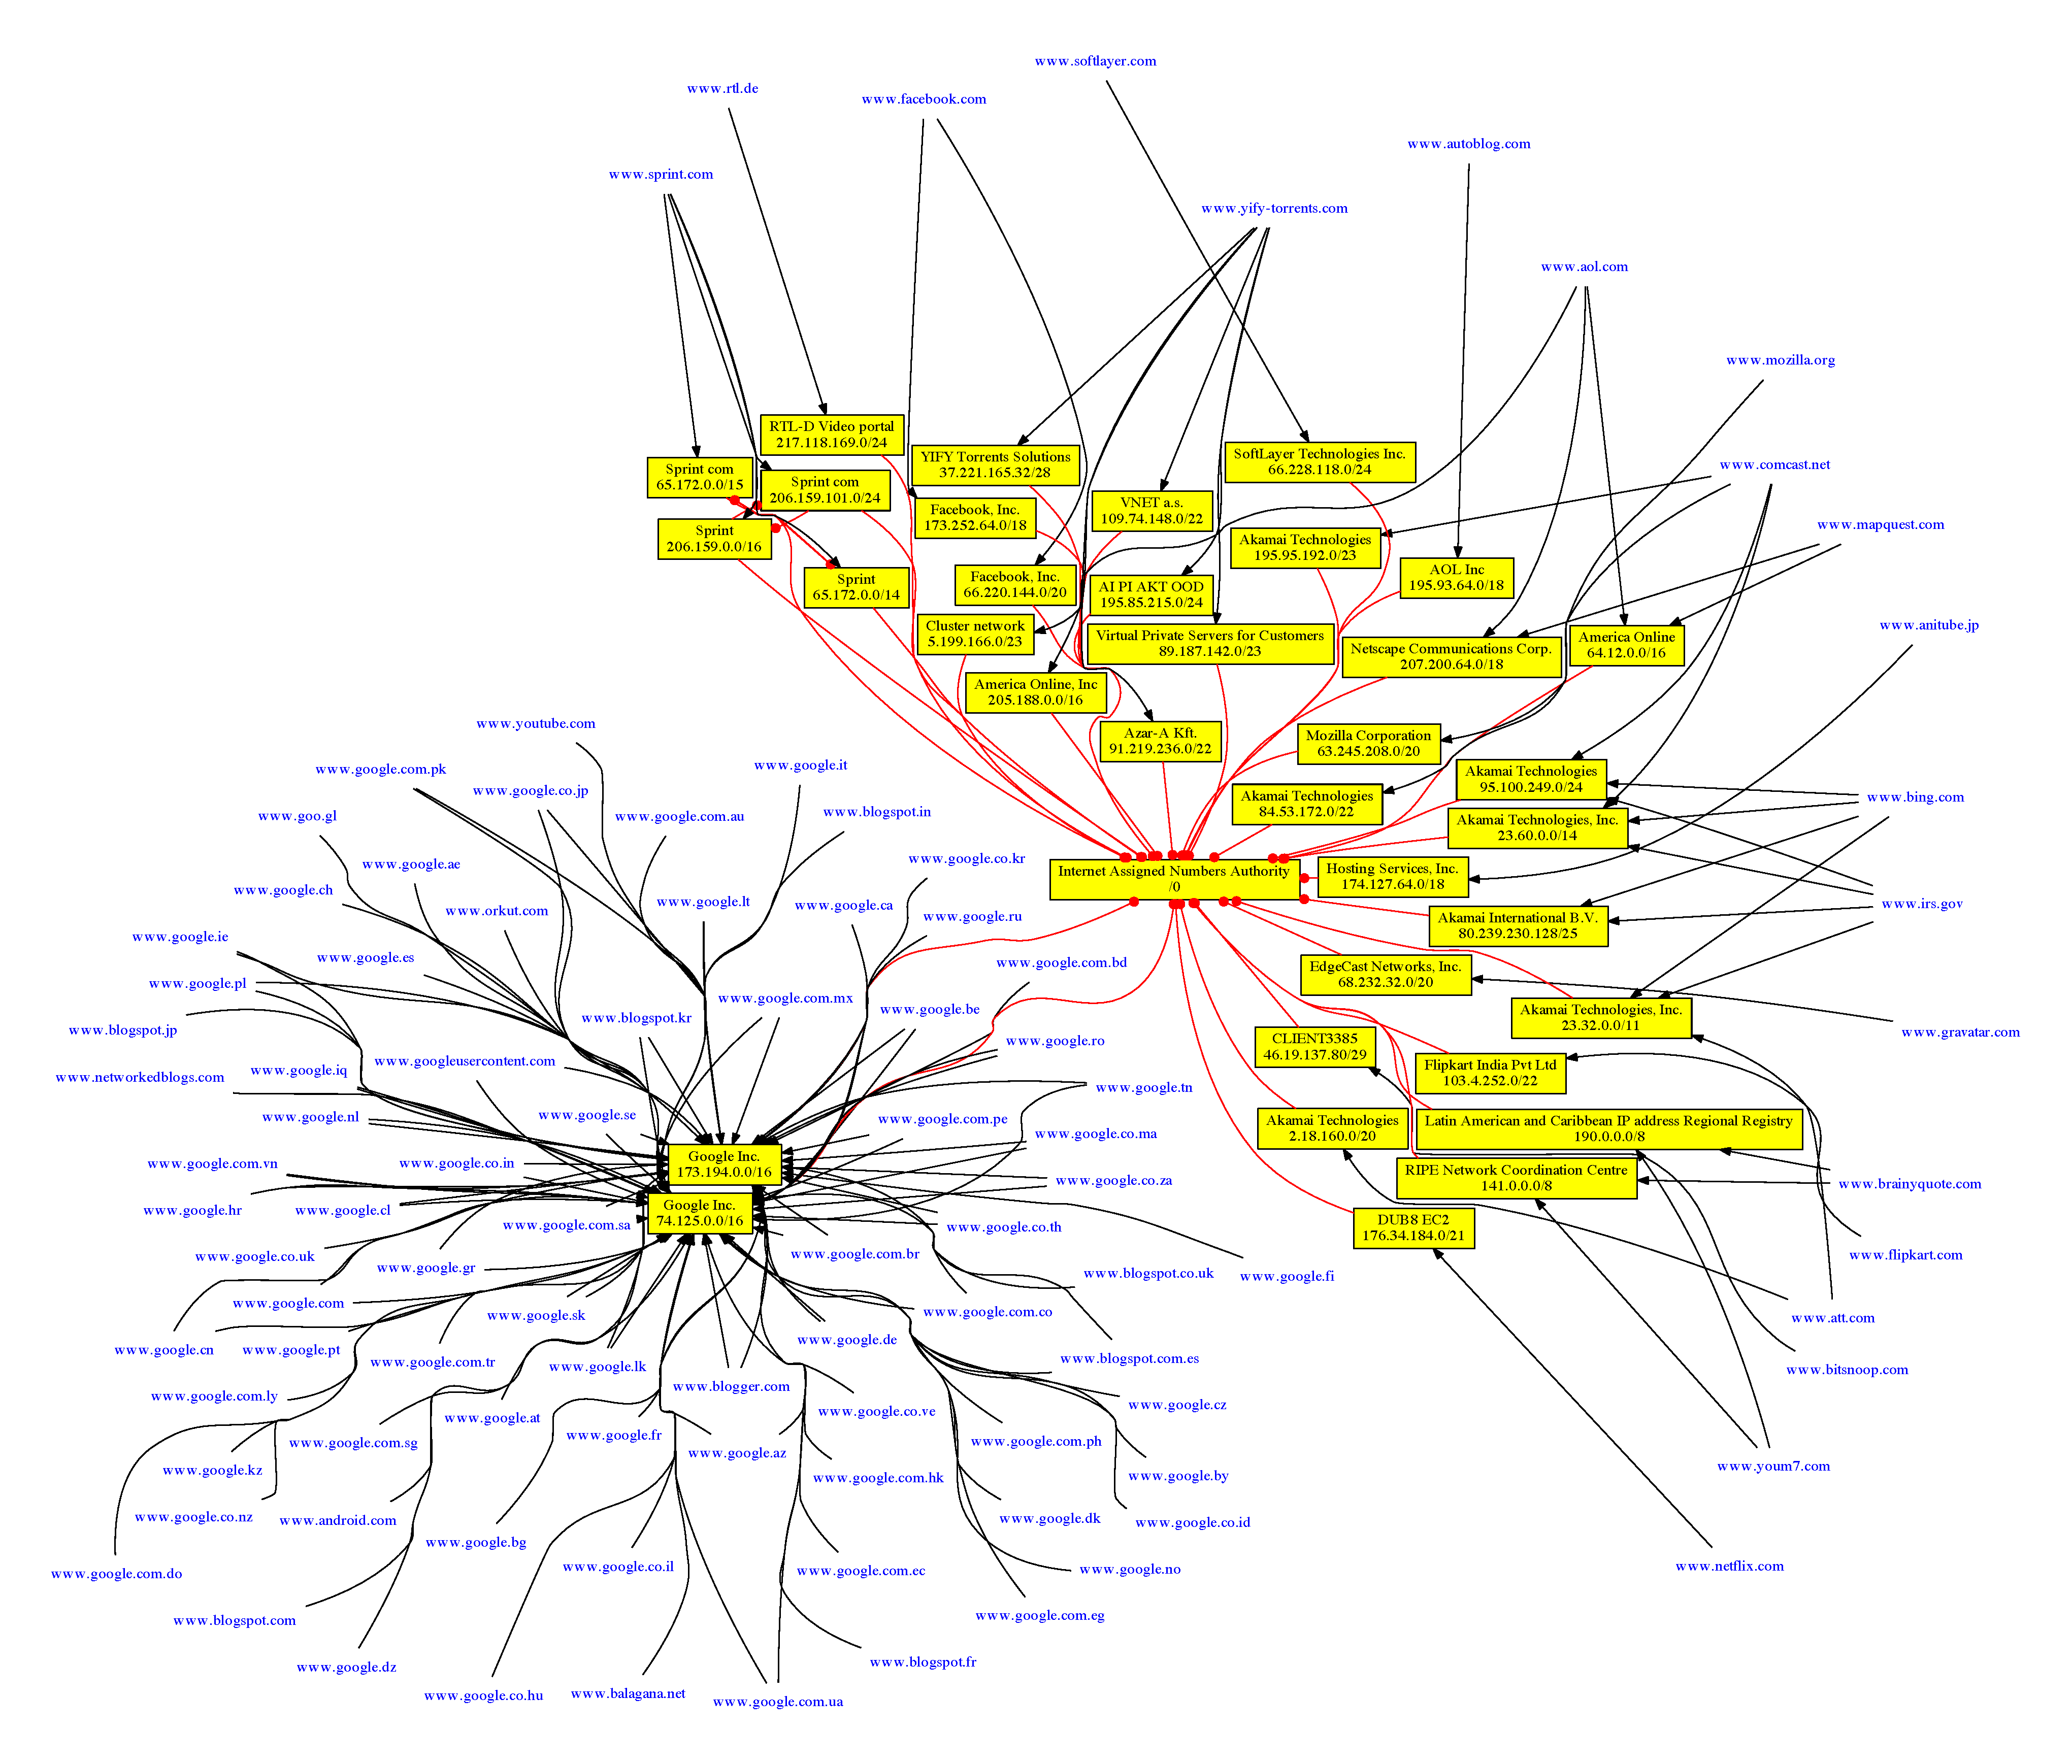
\includegraphics{figures/happy-v4cloud}}
  \end{minipage}
  \begin{minipage}[t]{0.50\textwidth}
    \centering
    \resizebox*{1.0\textwidth}{!}{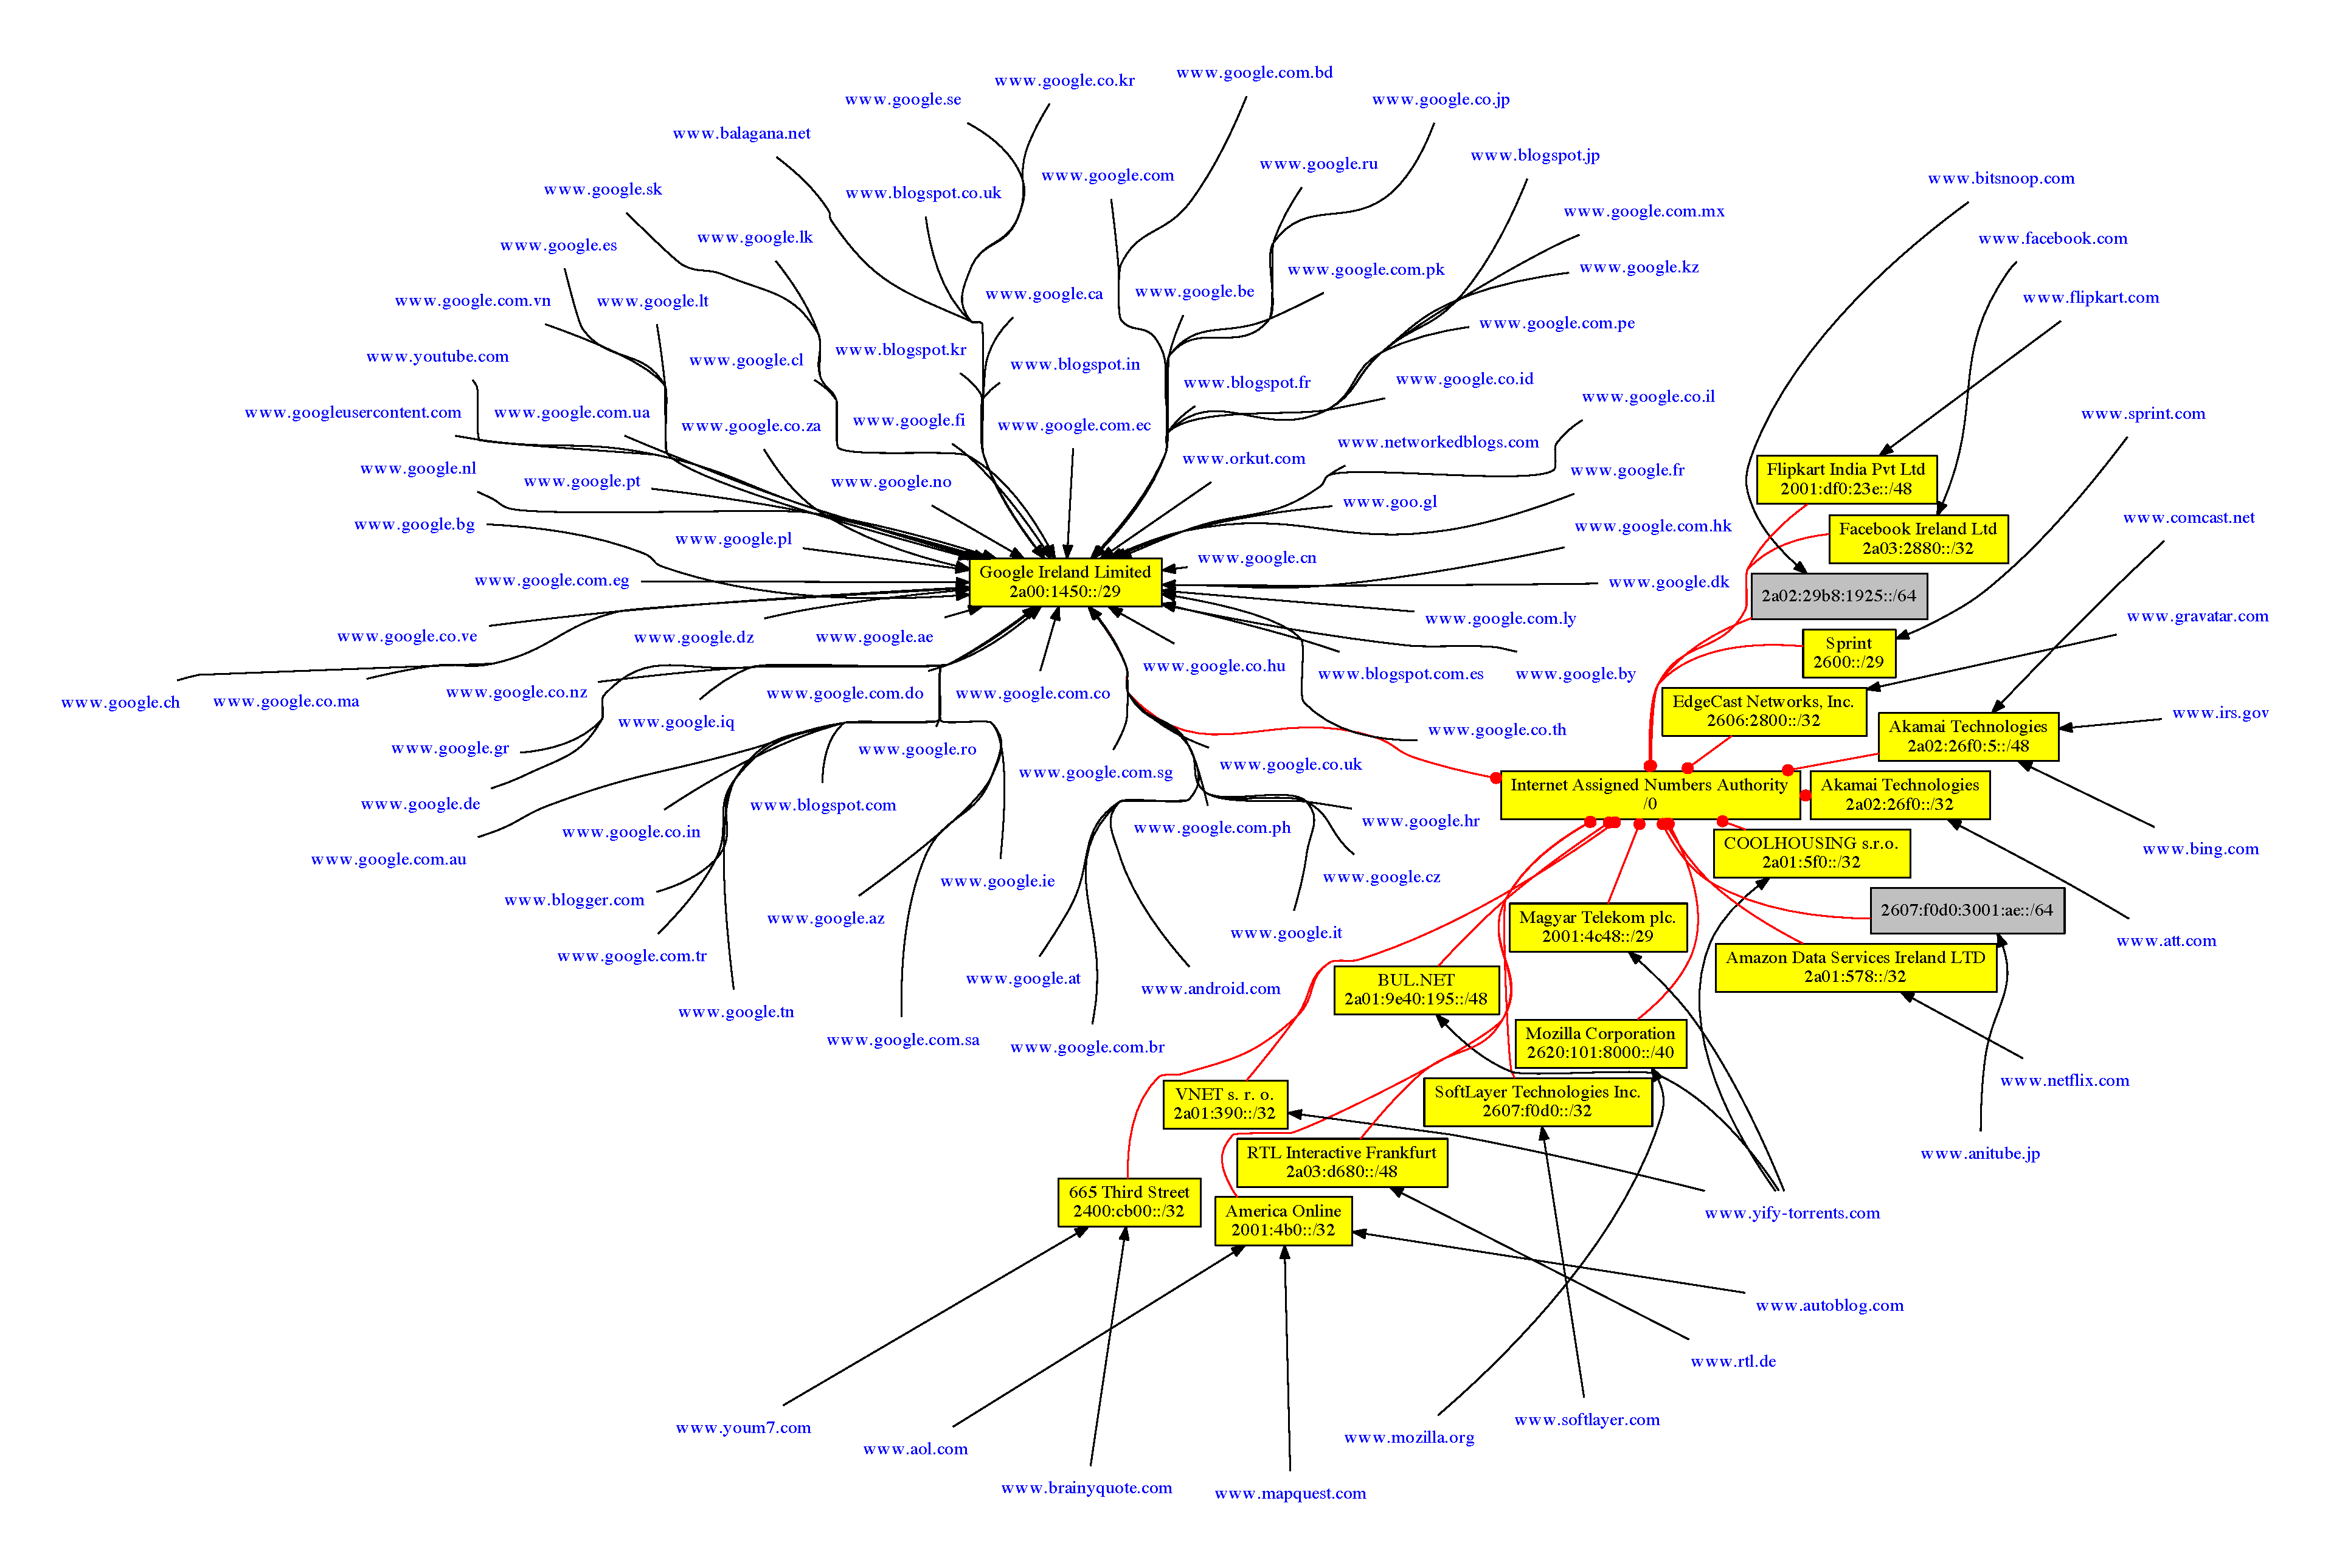
\includegraphics{figures/happy-v6cloud}}
  \end{minipage}
  \caption{\label{fig:v4-v6-cloud}An IPv4 and IPv6 aggregation cloud depicting
how most of the services centralize on core content delivery networks and
major cloud platforms}
\end{figure}

A preliminary result comparing the preference of a happy-eyeballed application
to IPv6 and IPv4 from two measurement points is shown in Fig.
\ref{fig:happy-v4-v6-compete}. The initial results show that happy eyeballs
prevents IPv6 access to Facebook, with only a 20\% chance to get to Google
related services over a Teredo Tunnel. The results look more promising on a
native IPv6 connection. It is important to note that adhering to the happy
eyeballs recommendation, IPv6 endpoints are allowed a 300ms chance to succeed.
A result comparing the time (mean and standard deviation) to establish a TCP
connection to each of the services from the same measurement points is shown
in Fig. \ref{fig:happy-v4-v6-mean-std}. The initial results show higher time
variances when connections are made over IPv6. In addition, it appears, some
of the related (and few of the unrelated) services show very similar
performances.  These services either resolve to the same endpoint or a set of
endpoints that belong to the same allocated prefix. Digging through the
\texttt{whois} information for each of the endpoints from their \ac{RIR} seems
to indicate that major portion of the services map to allocated prefixes owned
by popular organizations like Google and Akamai Technologies as shown in Fig.
\ref{fig:v4-v6-cloud}\footnote{A full resolution image is available at
  \url{https://gist.github.com/vbajpai/4730696}}

%As much as it is important to define and implement new tests on these
%measurement infrastructure, it is also equally pertinent to not only be able
%to install, update and delete these tests but also configure the entire suite
%of probes using a standardized protocol over the network. The \ac{NETCONF}
%protocol \cite{rfc6241} is particularly designed to cater to this problem.
%Towards this end, we have built a \ac{NETCONF} server for the OpenWRT platform
%using the \texttt{libnetconf}
%\footnote{\url{http://code.google.com/p/libnetconf/}} library and tested the
%implementation using our NETCONF Python API \texttt{ncclient}
%\cite{sbhushan:2009}. This will allow automated deployment of measurement
%tests and remote management of their startup configurations.

\label{sec:preliminaryresults}
\section{Conclusion}
We have performed a preliminary study on how IPv6 deployment may affect the
\ac{QoE} of Internet users. Using a large-scale measurement platform we want
to take this further, and define new metrics, measurement tests and data
analysis tools that help us understand the impact of network infrastructure
changes.
\label{sec:conclusion}
%----------------------------------------------------------------------



% bibliography
%----------------------------------------------------------------------
\bibliographystyle{splncs}
\bibliography{index}
%----------------------------------------------------------------------

\end{document}
